\documentclass{article}
\usepackage{graphicx} % Required for inserting images
\usepackage{geometry}
\usepackage{circuitikz}
\usepackage{siunitx}
\usepackage{CJKutf8}
\usepackage{amsmath}
\usepackage{amssymb}
\usepackage{caption}
\usepackage{float}
\usepackage{subcaption}
\geometry{top=10mm, left=20mm, a4paper}
\title{CMOS Operational Amplifier Report}
\author{梁程捷(B11901136),吳奕娃(B11901080)}
\date{}

\begin{document}
\begin{CJK*}{UTF8}{bkai}
\maketitle

%============Differential Amplifier====================
\section*{CMOS Operational Amplifier Small Signal Analysis}

\begin{figure}[H]
\begin{center}
    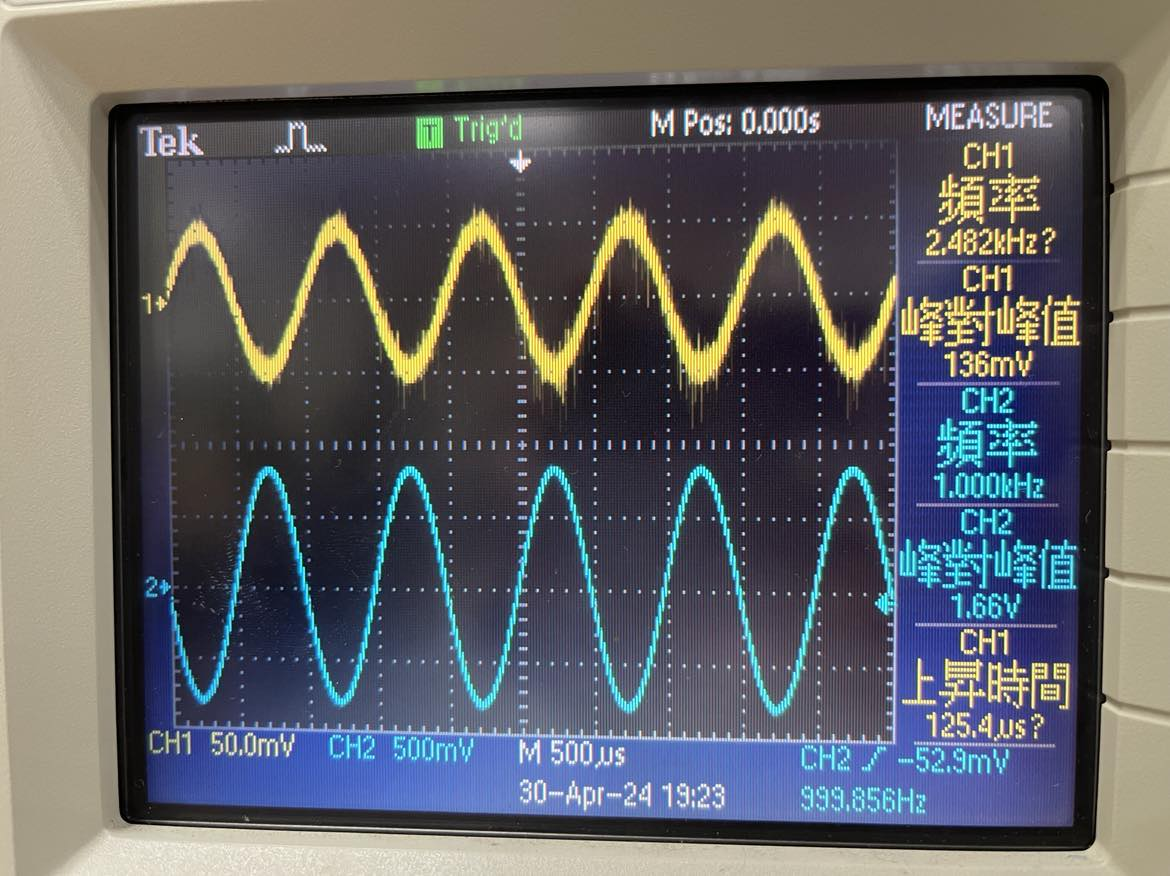
\includegraphics[scale = 0.2]{vo_n_vi_vtgraph.jpg}
    \caption{Waveforms of $V_i$ and $V_o$ in Y-t mode}
\end{center}
\end{figure}

\begin{minipage}{0.5\textwidth}
\begin{table}[H]
\begin{tabular}{|c|c|c||c|c|c|}
    \hline
    $f$ (\unit{\kilo\hertz}) &  $V_i$ (V)& $V_o$ (V) & $f$ (\unit{\kilo\hertz}) &  $V_i$ (V)& $V_o$ (V)\\
    \hline\hline
    1	    & 0.032 & 0.50 & 200    & 0.100 & 1.54   \\
    3       & 0.080 & 1.30 & 300    & 0.100 & 1.62   \\
    5	    & 0.070 & 1.12 & 500    & 0.100 & 1.84   \\
    7	    & 0.088 & 1.44 & 700    & 0.104 & 1.88   \\
    10	    & 0.100 & 1.62 & 800    & 0.106 & 1.68   \\
    30	    & 0.100 & 1.60 & 900    & 0.106 & 1.40   \\
    50	    & 0.100 & 1.58 & 950    & 0.108 & 1.26   \\
    70  	& 0.100 & 1.54 & \underline{\textbf{970}}  & \underline{\textbf{0.108}} & \underline{\textbf{1.20}}   \\
    100     & 0.100 & 1.56 & 1000   & 0.108 & 1.12   \\
    130     & 0.100 & 1.52 & 1500   & 0.106 & 0.44   \\
\hline
\end{tabular}
\caption{raw experimental data}
\end{table}
\end{minipage}\hspace{20mm}
\begin{minipage}{0.5\textwidth}
    \begin{figure}[H]    
        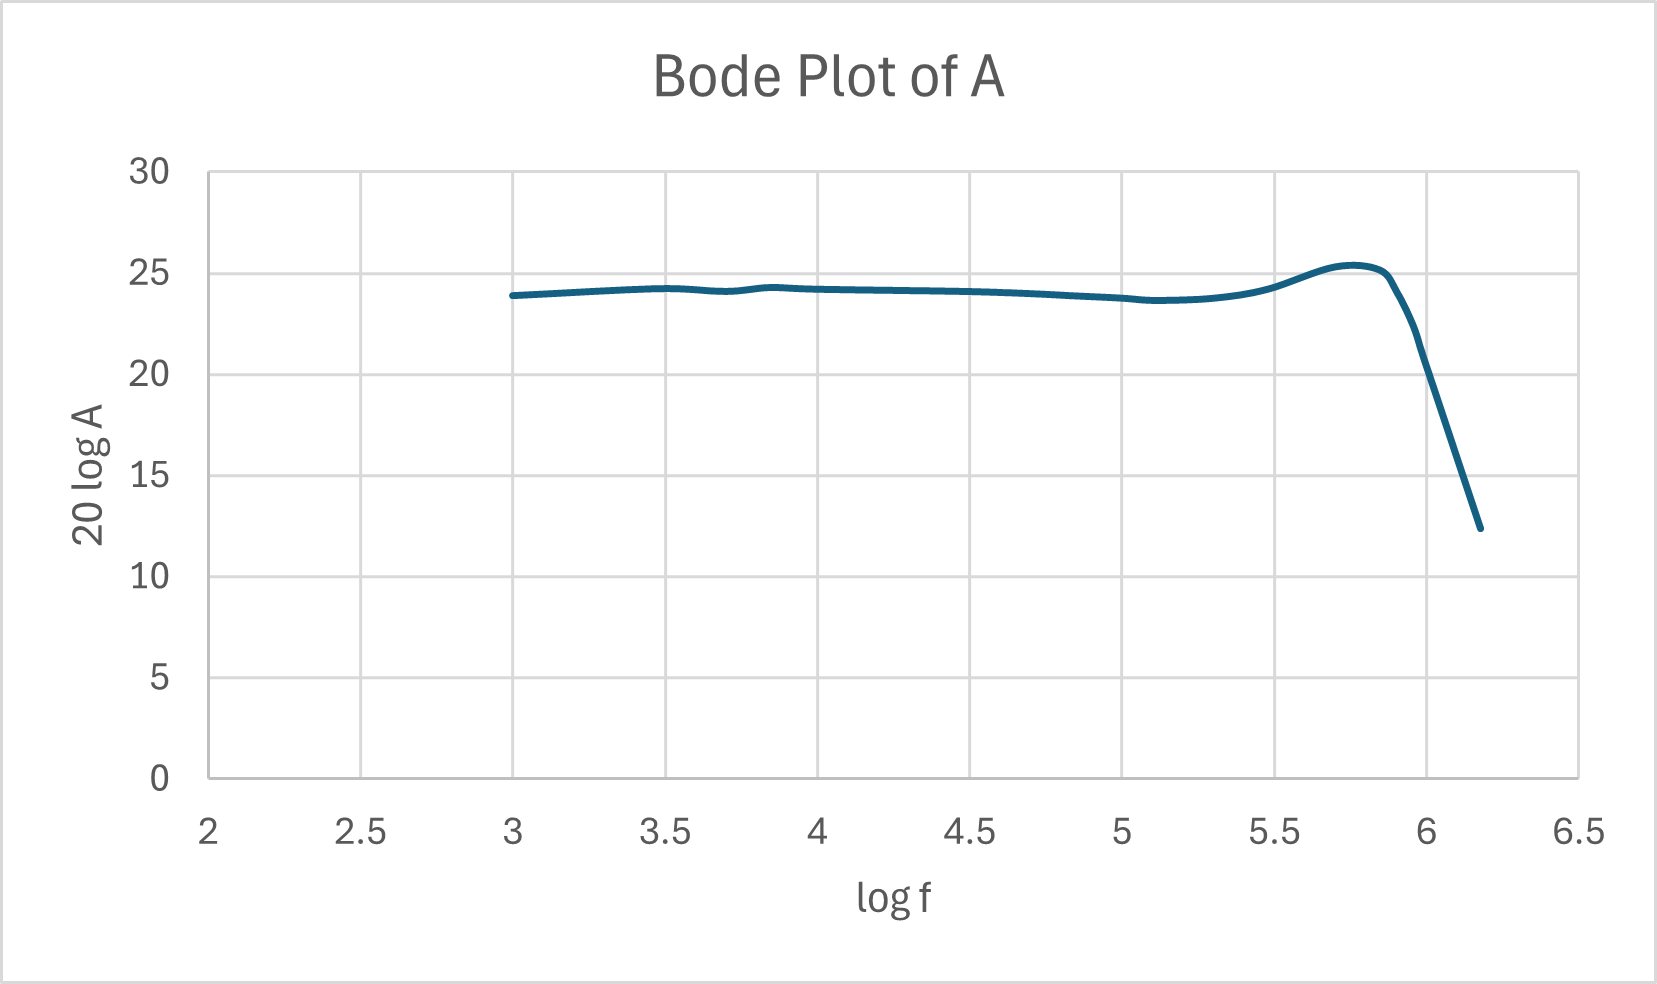
\includegraphics[scale=0.60]{bodeplotA.png}
        \caption{Bode Plot of $A$}
    \end{figure}
\end{minipage}
\vspace{3mm}\\
\textbf{3-dB frequency $f_{3dB} = 970$ \unit{\kilo\hertz}, bandwidth = 970 \unit{\kilo\hertz}}\\

\section*{Reflections}
\subsection*{梁程捷}
這次實驗的電路非常複雜,花了不少時間接電路,接了好幾次還是失敗,最後發現沒有接電供,哈哈。
\subsection*{吳奕娃}
這次的實驗感覺比以往困難不少,花了很多時間才做完,希望之後有機會練習以熟悉電路的接法。
\end{CJK*}
\end{document}
